\documentclass[10pt,mathserif]{beamer}

\usepackage[utf8]{inputenc}
\usepackage{lmodern}
\usepackage[T1]{fontenc}
\usepackage[spanish,activeacute]{babel}
\usepackage{mathtools}
\usepackage{amssymb}
\usepackage{graphicx}




%\usepackage{showkeys}
\usepackage{bbm}

%\usepackage{enumerate} 
\usepackage{setspace}
%\usepackage{hyperref}
\usepackage{listings,color}
\definecolor{mygreen}{rgb}{0,0.4,0}
\definecolor{myorange}{rgb}{0.88,0.43,0}
\definecolor{mybrown}{rgb}{0.5,0,0}
\definecolor{mygray}{rgb}{0.5,0.5,0.5}
\definecolor{mymauve}{rgb}{0.58,0,0.82}
\definecolor{probando}{rgb}{94,31,22}
\lstset{ %
  backgroundcolor=\color{white},   % choose the background color; you must add \usepackage{color} or \usepackage{xcolor}
  basicstyle=\footnotesize,        % the size of the fonts that are used for the code
  breakatwhitespace=false,         % sets if automatic breaks should only happen at whitespace
  breaklines=true,                 % sets automatic line breaking
  captionpos=b,                    % sets the caption-position to bottom
  commentstyle=\color{mygreen},    % comment style
  deletekeywords={...},            % if you want to delete keywords from the given language
  escapeinside={\%*}{*)},          % if you want to add LaTeX within your code
  extendedchars=true,              % lets you use non-ASCII characters; for 8-bits encodings only, does not work with UTF-8
  frame=single,	                   % adds a frame around the code
  keepspaces=true,                 % keeps spaces in text, useful for keeping indentation of code (possibly needs columns=flexible)
  keywordstyle=\color{blue},       % keyword style
  language=Octave,                 % the language of the code
  otherkeywords={*,...},           % if you want to add more keywords to the set
  numbers=none,                    % where to put the line-numbers; possible values are (none, left, right)
  numbersep=5pt,                   % how far the line-numbers are from the code
  numberstyle=\tiny\color{mygray}, % the style that is used for the line-numbers
  rulecolor=\color{black},         % if not set, the frame-color may be changed on line-breaks within not-black text (e.g. comments (green here))
  showspaces=false,                % show spaces everywhere adding particular underscores; it overrides 'showstringspaces'
  showstringspaces=false,          % underline spaces within strings only
  showtabs=false,                  % show tabs within strings adding particular underscores
  stepnumber=2,                    % the step between two line-numbers. If it's 1, each line will be numbered
  stringstyle=\color{mymauve},     % string literal style
  tabsize=2,	                   % sets default tabsize to 2 spaces
%  title=\lstname                   % show the filename of files included with \lstinputlisting; also try caption instead of title
}
%\newcommand{\xcal}[1]{\text{\usefont{OMS}{cmsy}{m}{n}#1}}
%\DeclareMathAlphabet{\mathpzc}{OMS}{cmex}{m}{n}
\DeclareMathAlphabet{\mathpzc}{OT1}{pzc}{m}{n}
%\DeclareMathAlphabet{\mathcalligra}{T1}{calligra}{m}{n}
%\newcommand{\mycal}{\usefont{OT1}{pzc}{m}{n}\fontsize{10}{12}\selectfont} 

\newcommand{\N}{\mathbbm{N}}
\newcommand{\R}{\mathbbm{R}}
\newcommand{\Rn}{\R^n}
\newcommand{\arr}{\rightarrow}
\newcommand{\bx}{\bar{x}}
\newcommand{\blambda}{\bar{\lambda}}
\newcommand{\bmu}{\bar{\mu}}
\newcommand{\cN}{\mathcal{N}}
\newcommand{\cT}{\mathcal{T}}
\newcommand{\cI}{\mathpzc{I}}
\newcommand{\cE}{\mathpzc{E}}
\newcommand{\cA}{\mathpzc{A}}
\newcommand{\la}{\langle}
\newcommand{\ra}{\rangle}
\newcommand{\deb}{\rightharpoonup}
%\usepackage[latin1]{inputec}
%\usetheme{Warsaw}
%\usecolortheme{crane}
%\usefonttheme{serif}
%\useoutertheme{shadow}
%\useinnertheme{rectangles}
%\mode<presentation>{\usetheme{Madrid}}
\mode<presentation>{\usetheme{Szeged}}%{Singapore}
\usecolortheme{rose}%{wolverine}%{seagull}%{whale}
%\usecolortheme[named=violet]{structure}%{seahorse}


\title{Trayectorias de tiempo óptimo para circuitos cerrados} 
\author{Autor: Iván Mandelman\\
Director: Damián Fernández}
\date{4 de diciembre de 2017}
\begin{document}
\frame{\titlepage} 
$\,$\\
%\tableofcontents{}
\section{Introducci\'on}

\begin{frame}

\begin{block}{De qué se trata? (Cómo es la onda)}
Las trayectorias de tiempo óptimo en circuitos cerrados son usadas, por ejemplo, para determinar el camino que debe seguir un vehículo en una carrera o el recorrido de un riel en una línea de producción. Desde el punto de vista matemático, se plantea un problema de minimización de un cierto funcional (representante del tiempo) en el espacio de las curvas cerradas y sujeto a condiciones propias del problema.
\end{block}


\pause

\begin{block}{Objetivo}
    Plantear y resolver el correspondiente problema de optimización.
\end{block}
\vspace{5cm}
\end{frame}

\section{Preliminares}

\begin{frame}
\begin{itemize}
    \item Geometría diferencial (curvas planas).
    \item Existencia de soluciones para problemas de optimización.
    \item Existencia de multiplicadores de Lagrange.
    \item Métodos numéricos para resolver problemas de optimización.
\end{itemize}
\end{frame}





\section{La trayectoria óptima}
\subsection{El ``Problema del TC''}
\begin{frame}


\begin{block}{Visualización}
Una manera simple de visualizar el problema que se quiere resolver, es  imaginar encontrarse en alguno de los circuitos del TC (turismo carretera), estos circuitos (o pistas), tienen un punto (o línea) de salida, que es el mismo que el de llegada, y el objetivo, es dar una determinada cantidad de ``vueltas'' en el menor tiempo posible. Es sensato entonces, decir que, encontrando una estrategia óptima para \emph{una} vuelta, se estará cumpliendo el objetivo antes mencionado.
\end{block}

\pause

\textcolor{mymauve}{No habrán restricciones en relación a la masa del vehículo (supondremos que nuestro vehículo tiene una masa ``puntual'') y el circuito será plano.}
\end{frame}



\begin{frame}

\begin{figure}[h!]
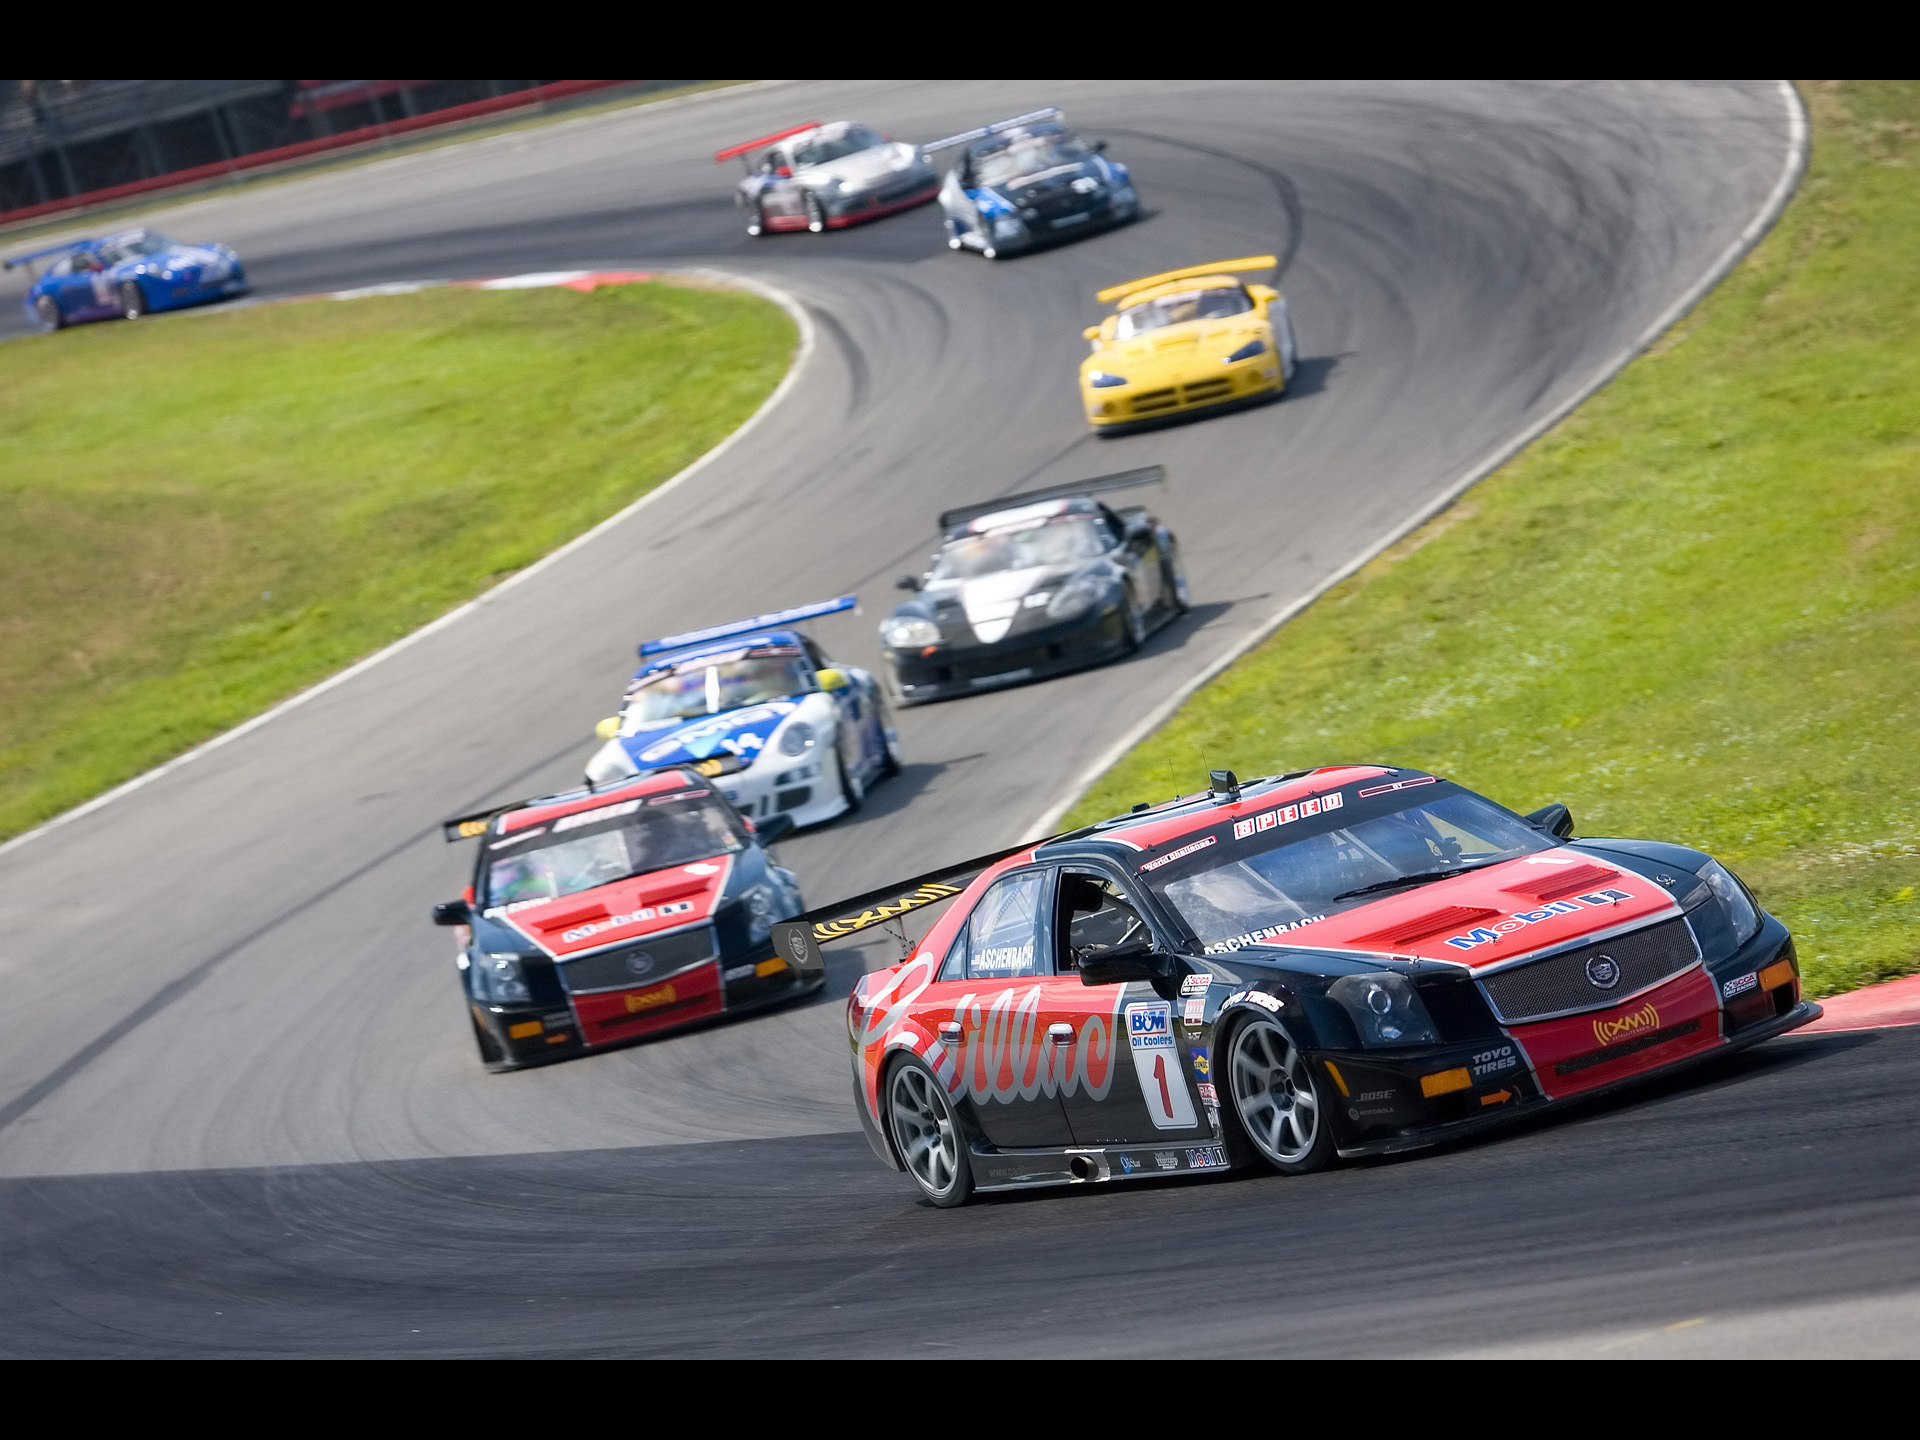
\includegraphics[scale=0.5]{Imagenes/The-dangers-of-race-car-driving.jpg}
\caption{Más visualización.}
\label{carreraTC}
\end{figure}


\end{frame}
\begin{frame}

Además, hay otras consideraciones a tener en cuenta:

\begin{itemize}
 \item \textcolor{red}{Mantenerse dentro de la pista, esto es indispensable pues se plantea que el terreno fuera de la pista es infranqueable en muchos casos.}
 
 \pause

  \item \textcolor{red}{La fricción de la pista, que regula los límites de la aceleración, y también, la trayectoria.}
  \end{itemize}

\pause

\begin{block}{}
Por lo tanto se plantea un problema de minimización, con determinadas restricciones. La función a minimizar es el tiempo, y algunas de las restricciones deberán ser la permanencia en pista y la fricción.
\end{block}

\end{frame}


\subsection{Formulación matemática}
\begin{frame}


\begin{block}{Objetivo}
Definir la función \textcolor{red}{tiempo final} $t_f$
\end{block}

\begin{block}{Restricciones}
\begin{itemize}
    \item \[
\textcolor{mymauve}{x(t)\in \mathcal{P}, \quad\forall t\in[0,t_f],}
\]
\item \begin{equation*}
 \textcolor{mymauve}{\left(\frac{a_t}{\mu_t}\right)^2+ \left(\frac{a_n}{\mu_n}\right)^2\leq g^2.} 
\end{equation*}
\end{itemize}
\end{block}

\begin{block}{}
\textcolor{mygreen}{Permanencia en pista y elipse de fricción.}
\end{block}

% El objetivo ahora es definir la función \textbf{tiempo final} $t_f$ que se quiere minimizar, sujeta a las dos condiciones mencionadas anteriormente. Matem\'aticamente la condici\'on de mantenerse dentro de la pista puede escribirse como


% donde $x$ es la trayectoria del vehículo y $\mathcal{P}$ es el conjunto de curvas que se mantienen dentro de la pista. 

% \pause

% La condici\'on de fricción regula las aceleraciones tangencial $a_t$ y normal $a_n$ para que cumplan

% donde $g$ es la acelaración de la gravedad, $\mu_t$ y $\mu_n$ son los coeficientes de rozamiento tangencial y normal, respectivamente. Tal condici\'on es conocida en la litaratura como \textcolor{red}{\textbf{elipse de fricción.}}

\end{frame}
\begin{frame}

Para facilitar las cuentas, reparametrizaremos la curva por longitud de arco. Se considera la función \textcolor{red}{\textbf{trayectoria}} de la curva como $x:[0,t_f]\mapsto \R^2$ tal que
\begin{equation*}\label{trayectoria}
\textcolor{myorange}{x(t) = p c(S(t)),}
\end{equation*}
con $c:[0,1]\arr\R^2$ tal que
\begin{equation*}\label{pla}
\textcolor{mybrown}{\left \|\frac{dc}{ds}(s)\right\|_{\R^2}=1,}
\end{equation*}
$p\in(0,+\infty)$ es la longitud de $x$ y $S:[0,t_f]\arr[0,1]$ es la función longitud de arco normalizada.
%pues
%\textcolor{mybrown}{\[
% \int_0^{t_f} \left\|\frac{dx}{dt}(t)\right\|_{\R^2} dt = p \int_0^{t_f} \frac{dS}{dt}(t)dt=p(S(t_f)-S(0))=p.
%\]}

\end{frame}
\begin{frame}

Definimos
  \begin{itemize}
      \item \textcolor{red}{\textbf{velocidad}} $\nu:[0,t_f]\arr\R^2$ tal que
      \textcolor{myorange}{\begin{equation*}
  \nu(t)=\frac{dx}{dt}(t)=p\frac{dc}{ds}(S(t))\frac{dS}{dt}(t), \label{velocidad}
\end{equation*}}
    \item \textcolor{red}{\textbf{rapidez}} (magnitud de la velocidad) $\tilde{v}:[0,t_f]\arr\R$ tal que
\textcolor{myorange}{\[
 \tilde{v}(t)=p\frac{dS}{dt}(t).
\]}
  \end{itemize}
   


Sea $T:[0,1]\arr [0,t_f]$ con $T(0)=0$, la inversa de $S$, definimos
\textcolor{myorange}{\begin{equation*}\label{v}
v(s)=\tilde v(T(s))=p\frac{dS}{dt}(T(s)). 
\end{equation*}}
Como $s=S(T(s))$, derivando en relaci\'on a $s$ obtenemos 
\textcolor{mybrown}{\begin{equation*}\label{auxdSdt}
1=\frac{dS}{dt}(T(s)) \frac{dT}{ds}(s)= \frac{1}{p} v(s)\frac{dT}{ds}(s), 
\end{equation*}}
\end{frame}
\begin{frame}
  por lo tanto
\textcolor{mybrown}{\[
 \frac{dT}{ds}(s)=\frac{p}{v(s)}.
\]}
Integrando, se obtiene que el tiempo final es
\textcolor{myorange}{\begin{equation*}\label{tiempo}
t_f=T(1)-T(0)=\int_{0}^{1} \frac{dT}{ds}(s) ds= \int_{0}^{1} \frac{p}{v(s)}ds.    
\end{equation*}}

\pause
Ahora, para obtener las aceleraciones (normal y tangencial) se calcula
\textcolor{mybrown}{\begin{equation*}\label{aceleracion}
\frac{d^2 x}{dt^2}(t)= p\frac{d^2 c}{ds^2}(S(t)) \left(\frac{dS}{dt}(t)\right)^2 + p\frac{dc}{ds}(S(t))\frac{d^2 S}{dt^2}(t),
\end{equation*}}
% donde en el primer t\'ermino se encuentra la informaci\'on de la aceleraci\'on normal y en segundo el de la aceleraci\'on tangencial. Esto puede demostrarse usando que $c$ est\'a parametrizada por longitud de arco y por lo tanto
% \textcolor{mybrown}{\[
%  0=\frac{d}{ds}1=\frac{d}{ds}\left\| \frac{dc}{ds}(s)\right\|_{\R^2}^2=2 \left\langle\frac{dc}{ds}(s) , \frac{d^2 c}{ds^2}(s)\right\rangle. 
% \]}
luego, la aceleración normal tiene magnitud
\textcolor{myorange}{\begin{equation*}\label{acelnormal}
a_n(s)=p\left(\frac{dS}{dt}(T(s))\right)^2\left\| \frac{d^2 c}{ds^2}(s) \right\|=\frac{1}{p} v(s)^2\left\| \frac{d^2 c}{ds^2}(s) \right\|_{\R^2}.
\end{equation*}}


\end{frame}
\begin{frame}
   Además
\[
\textcolor{mybrown}{ \frac{dv}{ds}(s)=p\frac{d^2 S}{dt^2}(T(s))\frac{dT}{ds}(s)=p\frac{d^2 S}{dt^2}(T(s))\frac{p}{v(s)}.}
\]
Por lo tanto la aceleración tangencial es
\[
\textcolor{myorange}{ a(s):=a_t(s)=p\frac{d^2 S}{dt^2}(T(s))=\frac{1}{p} v(s)\frac{d v}{ds}(s)=\frac{1}{p}\frac{d}{ds}\left(\frac{1}{2}v(s)^2\right)}
\]
Con esto, se obtiene que
\begin{equation*}\label{rel}
\textcolor{myorange}{p \int_0^s a(r)dr =\frac{1}{2}(v(s)^2-v(0)^2).} 
\end{equation*}
de donde
\begin{equation*}
\textcolor{myorange}{v(s)=\sqrt{2p \int_0^s a(r)dr + v_0^2}.}
\end{equation*}

\end{frame}
% \begin{frame}
% \textbf{OPCION 2}
% 
% Luego de unas cuentas con la derivada segunda de la trayectoria se obtiene
% \begin{itemize}
%     \item la magnitud de la aceleración normal
%     \textcolor{orange}{\begin{equation*}
% a_n(s)=p\left(\frac{dS}{dt}(T(s))\right)^2\left\| \frac{d^2 c}{ds^2}(s) \right\|=\frac{1}{p} v(s)^2\left\| \frac{d^2 c}{ds^2}(s) \right\|_{\R^2},
% \end{equation*}}
%     \item la aceleración tangencial
%     \textcolor{orange}{\[
%  a(s):=a_t(s)=p\frac{d^2 S}{dt^2}(T(s))=\frac{1}{p} v(s)\frac{d v}{ds}(s)=\frac{1}{p}\frac{d}{ds}\left(\frac{1}{2}v(s)^2\right),
% \]}
%     \item y la ecuación
%     \textcolor{orange}{\begin{equation*}
% p \int_0^s a(r)dr =\frac{1}{2}(v(s)^2-v(0)^2). 
% \end{equation*}}
% de donde
% \textcolor{orange}{\begin{equation*}
% v(s)=\sqrt{2p \int_0^s a(r)dr + v_0^2}
% \end{equation*}}
% 
% \end{itemize}
% 
% \end{frame}

\begin{frame}
\begin{block}{Problema}
Escribir una ecuación que represente la permanencia en pista.
\end{block}
\pause


\begin{figure}[h!]
\includegraphics[scale=0.8]{Imagenes/perm_pista}
\caption{$\alpha=$ curva interior, $\beta=$ curva exterior, $\kappa=$ ancho de pista.}
\label{perm_pista}
\end{figure}


\end{frame}





\begin{frame}

Considere que $\alpha:[0,1]\arr\R^2$ y $\beta:[0,1]\arr\R^2$ son las curvas que describen la calzada interna y externa de la pista, respectivamente, y sea $\kappa:[0,1]\arr(0,+\infty)$ el ancho de la calzada, o sea $\kappa(s)=\|\beta(s)-\alpha(s)\|_{\R^2}$. Se pedirá que para todo $s\in[0,1]$
\begin{equation*}
\textcolor{myorange}{\begin{array}{c}
 \|x(T(s))-\alpha(s)\|_{\R^2}^2 \leq \kappa(s)^2,\\[2mm]
 \|x(T(s))-\beta(s)\|_{\R^2}^2 \leq \kappa(s)^2.
\end{array}}
\end{equation*}
\pause
Por último, como las curvas (interna y externa) describirán un circuito plano, es necesario que no se intersequen consigo mismas, esto es, las curvas serán simples.
\vspace{5cm}
\end{frame}
\subsection{Problema de optimización}
\begin{frame}


Se puede comenzar ahora a escribir el problema de optimización.
Recapitulando lo anterior, identificamos las incógnitas:
\begin{itemize}
 \item la curva $c$,
 \item la aceleración tangencial $a$,
 \item la longitud de la curva $p$, y
 \item la velocidad inicial $v(0)$ a la cual llamaremos $v_0$.
\end{itemize}

\end{frame}

\begin{frame}

De las cuentas anteriormente realizadas surjen las restricciones:
\begin{enumerate}
\item la parametrización por longitud de arco de $c$.
\item La curva $c$ debe ser cerrada, luego $c(1)=c(0)$.
\item La velocidad y aceleraci\'on de $c$ deben ser curvas cerradas, entonces $\frac{dc}{ds}(1)=\frac{dc}{ds}(0)$, $\frac{d^2c}{ds^2}(1)=\frac{d^2c}{ds^2}(0)$.

\item La condición de la elipse de fricción.

\item La rapidez inicial y final deben ser iguales, por lo tanto $v(1)=v(0)$.

\item La aceleraci\'on tangencial inicial y final deben ser iguales, entonces $a(1)=a(0)$. 

\item \begin{equation*}
v(s)=\sqrt{2p \int_0^s a(r)dr + v_0^2}.
\end{equation*}

\item La permanencia en pista.
\end{enumerate}

\end{frame}
% \begin{frame}

% \[
% \begin{array}{rl}
% \displaystyle \mathop{\mathrm{minimizar}}_{(c,a,v,p,v_0)} & \displaystyle \int_{0}^{1} \frac{p}{v(s)}ds \\
%  \mathrm{sujeto \ a} & \left\|\frac{dc}{ds}(s)\right\|_{\R^2}^2-1=0,\,\forall s\in[0,1]\\[2mm]
%                      & c(1)-c(0)=0,\\[2mm]
%                      & \frac{dc}{ds}(1)-\frac{dc}{ds}(0)=0,\\[2mm]
%                      & \frac{d^2c}{ds^2}(1)-\frac{d^2c}{ds^2}(0)=0,\\[2mm]
%                      & v(1)-v_0=0,\\[2mm]
%                      & a(1)-a(0)=0,\\[2mm]
%                      &  \frac{1}{2}(v(s)^2-v_0^2)-p\int_0^s a(r)dr=0,\, \forall s\in[0,1],\\ [2mm]
%                      & \frac{1}{\mu_t^2} a(s)^2 + \frac{1}{\mu_n^2 p^2}v(s)^4\left\| \frac{d^2 c}{ds^2}(s) \right\|_{\R^2}^2-g^2\leq 0,\,\forall s\in[0,1],\\[2mm]
%                      &  \|pc(s)-\alpha(s)\|_{\R^2}^2-\kappa(s)^2 \leq 0,\,\forall s\in[0,1], \\[2mm]
%                      &  \|pc(s)-\beta(s)\|_{\R^2}^2-\kappa(s)^2 \leq 0,\, \forall s\in[0,1].
%   \end{array}
% \]
% donde $(c,a,v,p,v_0)\in H^2[0,1]^2\times L^2[0,1]\times L^2[0,1]\times\R_+\times \R_+$.
% \end{frame}
%Entonces el problema queda planteado de la siguiente manera
\begin{frame}{}
\vspace{-0.5cm}\begin{small}
\begin{equation*}
\begin{array}{rl}
\displaystyle \mathop{\mathrm{minimizar}}_{(c,a,p,v_0)} & \displaystyle \int_{0}^{1} \frac{p}{\sqrt{2p \int_0^s a(r)dr + v_0^2}}ds \\
 \mathrm{sujeto \ a} & \left\|\frac{dc}{ds}(s)\right\|_{\R^2}^2-1=0,\\[2mm]
                     & c(1)-c(0)=0,\\[2mm]
                     & \frac{dc}{ds}(1)-\frac{dc}{ds}(0)=0,\\[2mm]
                     & \frac{d^2c}{ds^2}(1)-\frac{d^2c}{ds^2}(0)=0,\\[2mm]
                     & \int_{0}^{1} a(r)dr=0,\\[2mm]
                     & a(1)-a(0)=0,\\[2mm]
                     & \frac{1}{\mu_t^2} a(s)^2 + \frac{1}{\mu_n^2 p^2}(2p \int_0^s a(r)dr + v_0^2)^2\left\| \frac{d^2 c}{ds^2}(s) \right\|_{\R^2}^2-g^2\leq 0,\,\forall s\in[0,1],\\[2mm]
                     &  \|pc(s)-\alpha(s)\|_{\R^2}^2-\kappa(s)^2 \leq 0,\,\forall s\in[0,1], \\[2mm]
                     &  \|pc(s)-\beta(s)\|_{\R^2}^2-\kappa(s)^2 \leq 0, \,\forall s\in[0,1].

  \end{array}
\end{equation*}
donde $(c,a,p,v_0)\in H^2[0,1]^2 \times L^2[0,1]\times \R_+\times \R_+$. 
\end{small}
\end{frame}
% \begin{frame}
% 
% donde $(c,a,p,v_0)\in H^2[0,1]^2 \times L^2[0,1]\times \R_+\times \R_+$. 
% 
% 
% \end{frame}




\section{Planteo final del problema}
\subsection{Dimensión infinita}
% \begin{frame}
% 
% \textbf{SECCION OBVIABLE}
% 
% 
% Para simplificar notación, reescribimos el problema anterior como
% \begin{equation*}
% \textcolor{red}{\begin{array}{rl}
% \displaystyle \mathop{\mathrm{minimizar}}_{x} & \displaystyle f(x) \\
% \mathrm{sujeto \ a} & G(x)\in K,\, x\in C
% \end{array}}
% \end{equation*}
% donde $f:X\arr \R$ con 
% \[
%  X=H^2[0,1]^2\times L^2[0,1]\times \R_+ \times \R_+,
% \]
% tal que para $x=(c,a,p,v_0)\in X$,
% $$
% \textcolor{mymauve}{f(x)=\int_{0}^{1} \frac{p}{v(s)}ds.}
% $$
% 
% Las restricciones $G:X\arr Z$ donde
% \[
% Z=L^2[0,1]\times \R^2\times \R\times \R\times \R^2\times \R^2\times L^2[0,1] \times L^2[0,1]^2 \times \R,
% \]
% 
% 
% \end{frame}

\begin{frame}
Para simplificar notación, reescribimos el problema anterior como
\begin{equation*}
\textcolor{red}{\begin{array}{rl}
\displaystyle \mathop{\mathrm{minimizar}}_{x} & \displaystyle f(x) \\
\mathrm{sujeto \ a} & G(x)\in K,\, x\in C
\end{array}}
\end{equation*}
donde $f:X\arr \R$, $G:X\arr Z$, $C\subset X$ y $K\subset Z$, con
\begin{eqnarray*}
 X&=&H^2[0,1]^2\times L^2[0,1]\times \R \times \R,\\
C&=&H^2[0,1]^2\times L^2[0,1]\times \R_+ \times \R_+,\\
Z&=&L^2[0,1]\times \R^2\times \R\times \R\times \R^2\times \R^2\times L^2[0,1] \times L^2[0,1]^2 \times L^2[0,1]^2,\\
K&=&\{0\}\times \{0\}\times \{0\}\times \{0\}\times \{0\}\times \{0\}\\
   &&\times (-L^2[0,1]_+) \times (-L^2[0,1]_+) \times (-L^2[0,1]_+).
\end{eqnarray*}
Para $x=(c,a,p,v_0)\in X$ las funciones se definen
$$
\textcolor{mymauve}{f(x)=\int_{0}^{1} \frac{p}{v(s)}ds,}
$$
\end{frame}

\begin{frame}
y \textcolor{red}{$G=(G_1,G_2,G_3,G_4,G_5,G_6,G_7,G_8,G_9)$}, tal que
\begin{small}
\begin{eqnarray*}
 G_1(x)(s)&=&\left\|\frac{dc}{ds}(s)\right\|_{\R^2}^2-1,\quad \mbox{p.p. }s\in(0,1)\\
 G_2(x)&=&c(1)-c(0),\\
 G_3(x)&=&\int_{0}^{1} a(r)dr,\\
 G_4(x)&=&a(1)-a(0),\\
 G_5(x)&=&\frac{dc}{ds}(1)-\frac{dc}{ds}(0),\\
 G_6(x)&=&\frac{d^2c}{ds^2}(1)-\frac{d^2c}{ds^2}(0),\\
 G_7(x)(s)&=&\frac{1}{\mu_t^2} a(s)^2 + \frac{1}{\mu_n^2 p^2}v(s)^4\left\| \frac{d^2 c}{ds^2}(s) \right\|_{\R^2}^2-g^2,\quad \mbox{p.p. }s\in(0,1),\\
 G_8(x)(s)&=&\|pc(s)-\alpha(s)\|_{\R^2}^2-\kappa(s)^2, \quad \mbox{p.p. }s\in(0,1),\\
 G_9(x)(s)&=&\|pc(s)-\beta(s)\|_{\R^2}^2-\kappa(s)^2, \quad \mbox{p.p. }s\in(0,1).
\end{eqnarray*}
\end{small}
\end{frame}
% \begin{frame}
%  
% \begin{eqnarray*}
%   G_8(x)(s)&=&\|pc(s)-\alpha(s)\|_{\R^2}^2-\kappa(s)^2, \quad \mbox{p.p. }s\in(0,1)\\
%  G_9(x)(s)&=&\|pc(s)-\beta(s)\|_{\R^2}^2-\kappa(s)^2, \quad \mbox{p.p. }s\in(0,1).
% \end{eqnarray*}
% 
% 
% 
% Adem\'as, $C\subset X$ y $K\subset Z$, dados por
% \begin{equation*}
%     \begin{array}{lll}
%       C&=&H^2[0,1]^2\times L^2[0,1]\times \R_+ \times \R_+,\\
%    K&=&\{0\}\times \{0\}\times \{0\}\times \{0\}\times \{0\}\times \{0\}\\
%    &&\times (-L^2[0,1]_+) \times (-L^2[0,1]_+) \times (-L^2[0,1]_+).
%     \end{array}
% \end{equation*}
% 
% 
% %\begin{eqnarray*}
% %C&=&H^2[0,1]^2\times L^2[0,1]\times \R_+ %\times \R_+,\\
% %K&=&\{0\}\times \{0\}\times \{0\}\times %\{0\}\times \{0\}\times \{0\}\times (-L^2[0,1]_+) \times (-L^2[0,1]_+) \times (-L^2[0,1]_+).
% %\end{eqnarray*}
% \end{frame}






\subsection{Dimensión finita}
\begin{frame}
\frametitle{Discretización}

Se utilizará el \textcolor{red}{\texttt{método de elementos finitos espectrales}}, donde se aproximan los espacios involucrados utilizando el generado por una cantidad finita de ciertos polinomios trigonométricos. 


Se aproximará el espacio 
\begin{itemize}
    \item $X=H^2[0,1]^2\times L^2[0,1]\times \R \times \R$\quad por $\quad\textbf{X}=V^2\times V\times \R\times \R$,
    
    con $\, V=\mbox{span}\left\{\varphi_j,\ j=1,\ldots, n\right\}$.
\end{itemize}

Donde se toman las siguientes funciones base
\begin{eqnarray}\label{funbase}
\varphi_j(t)&=&\left\{ \begin{array}{ll}
\frac{1}{2}, & \mbox{ si}\quad j=1,\\
\cos(2\pi kt), & \mbox{ si}\quad j=2k+1,\\
\mathrm{sen}(2\pi kt), & \mbox{ si}\quad j=2k,
\end{array}
\right.\mbox{para } k=1,\ldots,m,
\end{eqnarray}
con $n=2m+1$. 
\end{frame}
\begin{frame}
\begin{itemize}
    \item Para las coordenadas de $Z$ que se encuentran en $\R$, la función base que se utilizará es el número real $1$, pues span$\{1\}=\R$.
    \item En las coordenadas funcionales de $Z$ se aproximarán las funciones por su valor en una malla de $n+1$ puntos entre $0$ y $1$ dados por 
    \textcolor{red}{$$s_i=\frac{i-1}{n} \mbox{ para } i=1,\ldots,n+1,$$}
     para esto, se usará la función 
     $$\textcolor{mymauve}{\delta_{s_i}:C_c^\infty[0,1]\arr\R, \mbox{ tal que } \la\delta_{s_i},f\ra=f(s_i).}$$
     
\end{itemize}

 \pause

\begin{block}{Teorema}
Si $0=\displaystyle\sum_{l=1}^n\lambda_l\varphi_l(s_j)$ para $j=1,\ldots,n$ entonces $\lambda_l=0$ para $l=1,\ldots,n$.
\end{block}

\end{frame}
\begin{frame}

Por lo tanto escribimos

\begin{itemize}
    \item \textcolor{mymauve}{$$x=(c_1,c_2,a,p,v_0)\approx\hat{x}=\left(\sum_{k=1}^n\texttt{c}^1_k\varphi_k, \sum_{k=1}^n\texttt{c}^2_k\varphi_k,\sum_{i=1}^n\texttt{a}_i\varphi_i, p, v_0\right),$$}
    
    \item entonces, en el problema discretizado, la nueva variable es
    \textcolor{red}{$$\texttt{x}=(\texttt{c}^1,\texttt{c}^2,\texttt{a},p,v_0)\in\R^{3n+2}.$$} y podemos escribir
    \item \textcolor{mygreen}{$$\texttt{v}(s)=\sqrt{2p\int_0^s \sum_{i=1}^n\texttt{a}_i\varphi_i(r)dr +v_0^2},$$}
    \item \textcolor{blue}{$$f(x)\approx\texttt{f}(\texttt{x}):=f(\hat x)=\int_0^1 \frac{p}{\texttt{v}(s)}ds.$$}
    
\end{itemize}

\end{frame}
\begin{frame}

Ahora aproximamos las funciones de restricción, separando los casos de aquellas que llegan a $\R$ y las que llegan a $L^2[0,1]$.
\begin{itemize}
    \item \textcolor{red}{$$\texttt{G}_r(\texttt{x}):=G_r(\hat x),\quad r=2,3,4,5,6,$$}
    \item \textcolor{mygreen}{$$(\texttt{G}_r)_{i}(\texttt{x}):=\langle G_r(\hat x) , \delta_{s_i}\rangle,\,i=1,\ldots,n; \quad r=1,7,8,9.$$}
\end{itemize}

\begin{block}{}
Como las funciones base son periódicas, es decir que $\varphi_j(0)=\varphi_j(1)\, \forall j$, se tiene que $\texttt{G}_2,\texttt{G}_4,\texttt{G}_5\mbox{ y }\texttt{G}_6$ son iguales a 0, por lo que esas restricciones se cumplen automáticamente.
\end{block}
\end{frame}
\begin{frame}
\begin{footnotesize}
Luego, el planteo del problema queda de la siguiente forma
\begin{equation*}
\begin{array}{ll}
&\hspace{-1cm}\displaystyle \mathop{\mathrm{minimizar}}_{(\texttt{c}^1,\texttt{c}^2,\texttt{a},p,v_0)}  \texttt{f}(\texttt{x})=\int_0^1\frac{p}{\sqrt{2p\int_0^s \sum_{i=1}^n\texttt{a}_i\varphi_i(r)dr +v_0^2}}\\
\hspace{-0.5cm} \mathrm{s.a} &\displaystyle \left\|\left(\sum_{k=1}^n\texttt{c}^1_k\varphi'_k(s_j), \sum_{k=1}^n\texttt{c}^2_k\varphi'_k(s_j)\right)\right\|_{\R^2}^2-1=0,\\[2mm]
                     &\displaystyle \int_{0}^{1} \sum_{i=1}^n\texttt{a}_i\varphi_i(r)dr=0,\\[2mm]
                     &\displaystyle \frac{1}{\mu_t^2} \left(\sum_{i=1}^n\texttt{a}_i\varphi_i(s_j)\right)^2 + \frac{1}{\mu_n^2 p^2}\texttt{v}(s_j)^4\left\| \left(\sum_{k=1}^n\texttt{c}^1_k\varphi_k''(s_j), \sum_{k=1}^n\texttt{c}^2_k\varphi_k''(s_j)\right) \right\|_{\R^2}^2-g^2\leq 0,\,\\[2mm]
                     &\displaystyle  \left\|p\left(\sum_{k=1}^n\texttt{c}^1_k\varphi_k(s_j), \sum_{k=1}^n\texttt{c}^2_k\varphi_k(s_j)\right)-\alpha(s_j)\right\|_{\R^2}^2-\kappa(s_j)^2 \leq 0,\, \\[2mm]
                     &\displaystyle  \left\|p\left(\sum_{k=1}^n\texttt{c}^1_k\varphi_k(s_j), \sum_{k=1}^n\texttt{c}^2_k\varphi_k(s_j)\right)-\beta(s_j)\right\|_{\R^2}^2-\kappa(s_j)^2 \leq 0, \,\\[2mm]
                     & p\geq 0,\ v_0\geq 0,

  \end{array}
\end{equation*}
%donde las restricciones (salvo la segunda) deben cumplirse para cada $j=1,\ldots l$.
\end{footnotesize}
\end{frame}
\begin{frame}

\frametitle{Existencia de solución}
\begin{block}{Teorema}
Sea 
$$S=\{\texttt{x}\in\R^{3n+2}\mid \texttt{G}(\texttt{x})\in \texttt{K}\}\mbox{ y }R=\{\texttt{x}\in\R^{3n+2}\mid \texttt{f}(\texttt{x})\leq \texttt{f}_0\},$$
donde $\texttt{f}_0=\texttt{f}(\texttt{x}_0)$ para algún $\texttt{x}_0\in S$. Entonces el conjunto $S\cap R$ es compacto no vacío.
\end{block}



% Para probar la existencia de solución de el problema \eqref{pdisfinal}, observe que la función $\texttt{f}$ claramente es continua, por lo tanto si para un punto factible $\texttt{x}_0$ dado, el conjunto $\{\texttt{x}\in S\mid \texttt{f}(\texttt{x})\leq \texttt{f}(\texttt{x}_0)\}$ es compacto, entonces el Corolario \ref{solglobalfinita} nos garantiza la existencia de solución. Se demostrará entonces, que este conjunto es compacto. Para simplificar notación, sea 
% $$R=\{\texttt{x}\in\R^{3n+2}\mid \texttt{f}(\texttt{x})\leq \texttt{f}_0\},$$
% donde $\texttt{f}_0=\texttt{f}(\texttt{x}_0)$.
% \begin{teo}
% El conjunto $S\cap R$ es compacto no vacío.
% \end{teo}
\end{frame}
\section{Resultados computacionales}


\begin{frame}
% \begin{block}{}
% Para todos los problemas la discretización de las funciones se realizó tomando $n=113$ y la aceleración de la gravedad se definió como $g=9.8$. Las constantes de rozamiento $\mu_n$ y $\mu_t$ como las calzadas interna $\alpha$ y externa $\beta$ se detallarán para cada tipo de pista.
% \end{block}
\begin{block}{}
Se utilizó el algoritmo \textcolor{blue}{SQP} del programa \textcolor{mymauve}{fmincon} de MATLAB para resolver el problema discretizado.

Las curvas iniciales se mostrarán en color \textcolor{mygreen}{verde} y las óptimas obtenidas por el algoritmo en \textcolor{red}{rojo}.
\end{block}

% En todos los experimentos, la curva inicial se definió como $\gamma=\frac{1}{2}\alpha+\frac{1}{2}\beta$ tomando $p$ como su longitud y tomando $\texttt{c}^1_k,\, \texttt{c}^2_k$ de manera que $\left(\sum_{k=1}^n\texttt{c}^1_k\varphi_k, \sum_{k=1}^n\texttt{c}^2_k\varphi_k\right)=\frac{1}{p}\gamma$, la acelaración inicial se definió constantemente cero, i.e., $\texttt{a}_i=0$ y la velocidad inicial $v_0$ se definió de manera que la restricción de fricción sea satisfecha. 
\end{frame}
\subsection{Pista circular}
\begin{frame}

\begin{figure}[h!]
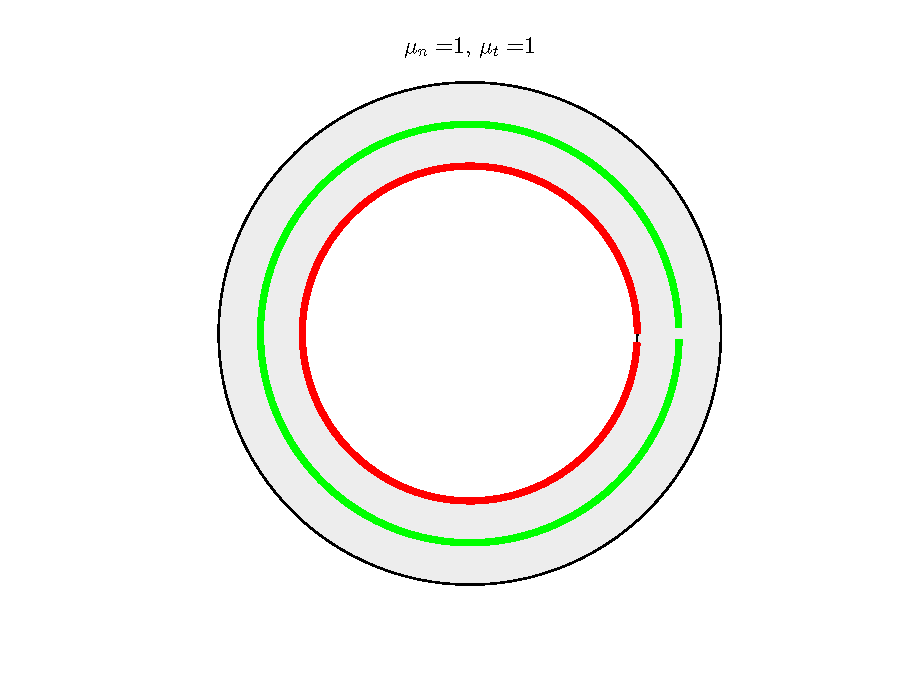
\includegraphics[scale=0.7]{graficos/circular/trayectoria1}
\end{figure}
\end{frame}
\begin{frame}
\begin{figure}[h!]
\begin{tabular}{cc}
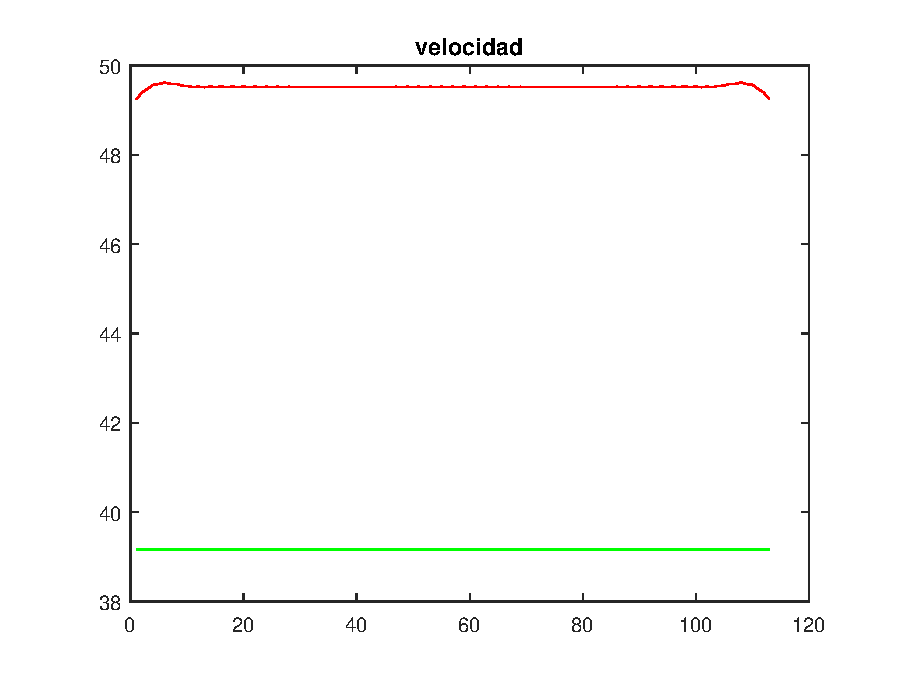
\includegraphics[scale=0.36]{graficos/circular/velocidad1} &
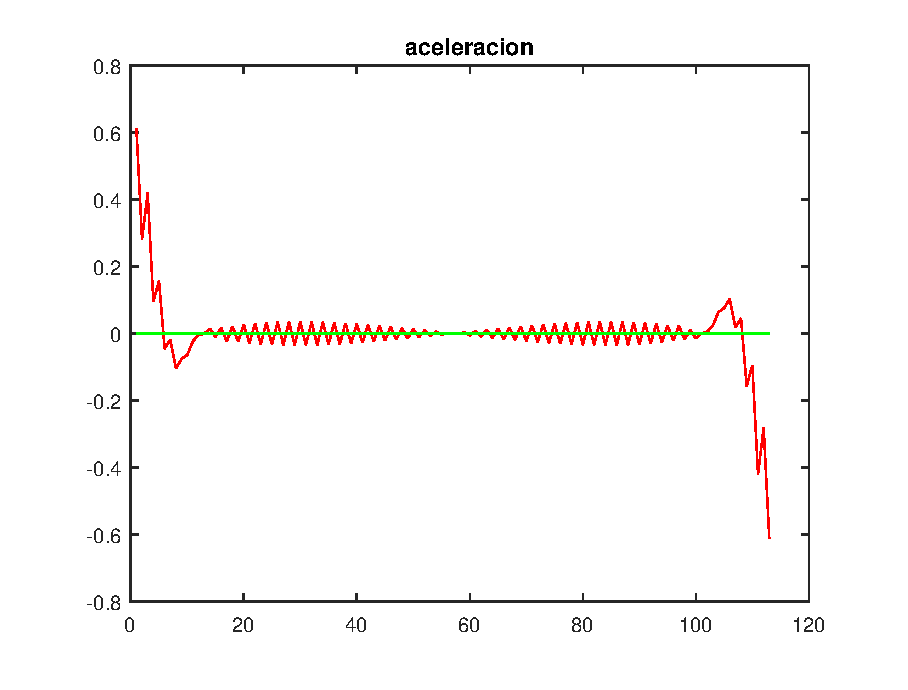
\includegraphics[scale=0.36]{graficos/circular/aceleracion1}
\end{tabular}
\label{circ1}
\end{figure}


\end{frame}

\begin{frame}

\begin{figure}[h!]
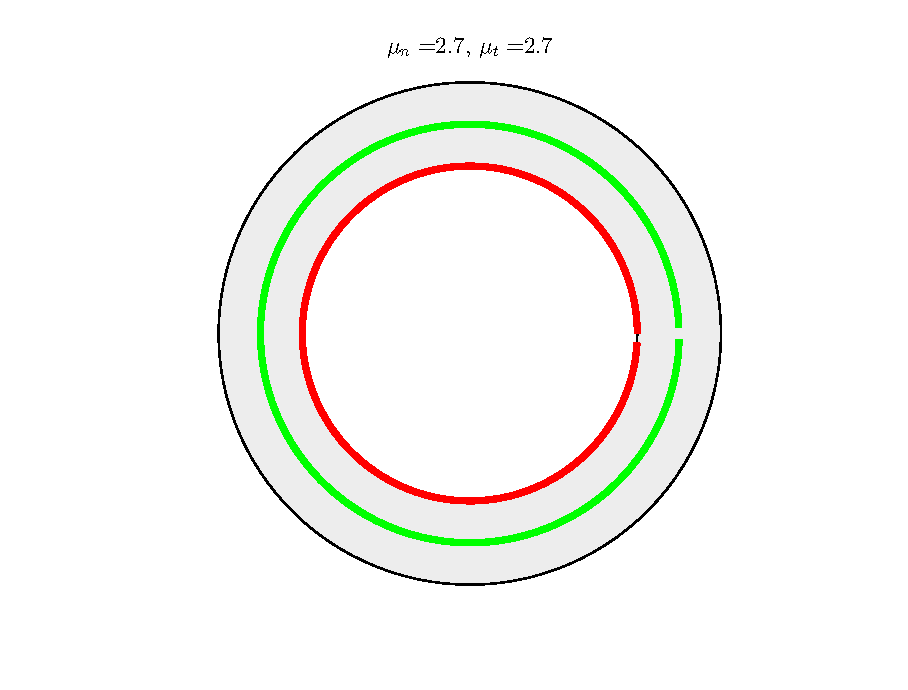
\includegraphics[scale=0.7]{graficos/circular/trayectoria2}
\end{figure}
\end{frame}
\begin{frame}
\begin{figure}[h!]
\begin{tabular}{cc}
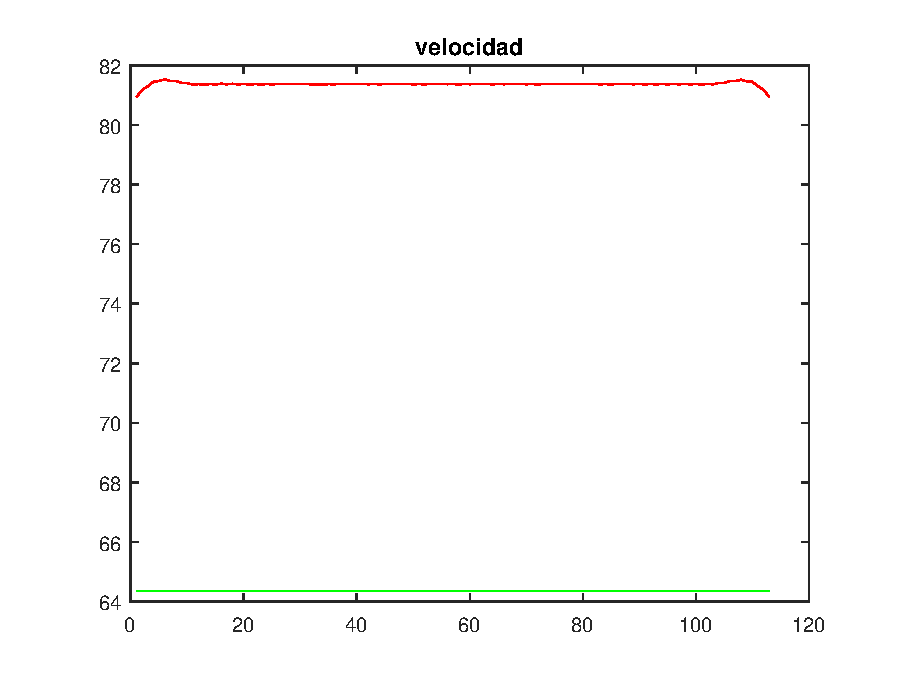
\includegraphics[scale=0.36]{graficos/circular/velocidad2} &
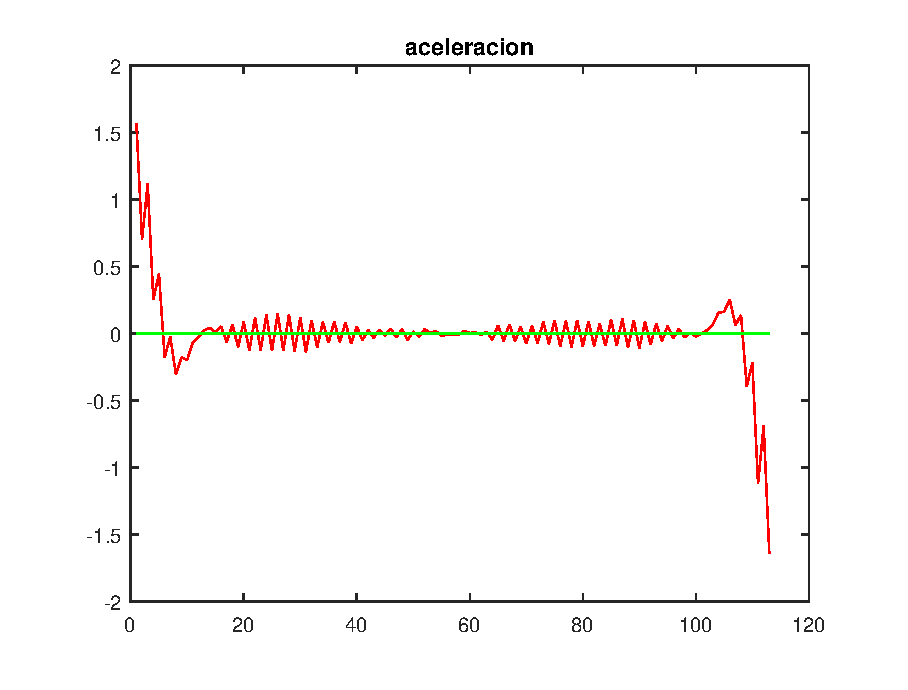
\includegraphics[scale=0.36]{graficos/circular/aceleracion2}
\end{tabular}

\label{circ2}
\end{figure}


\end{frame}


\begin{frame}

\begin{figure}[h!]
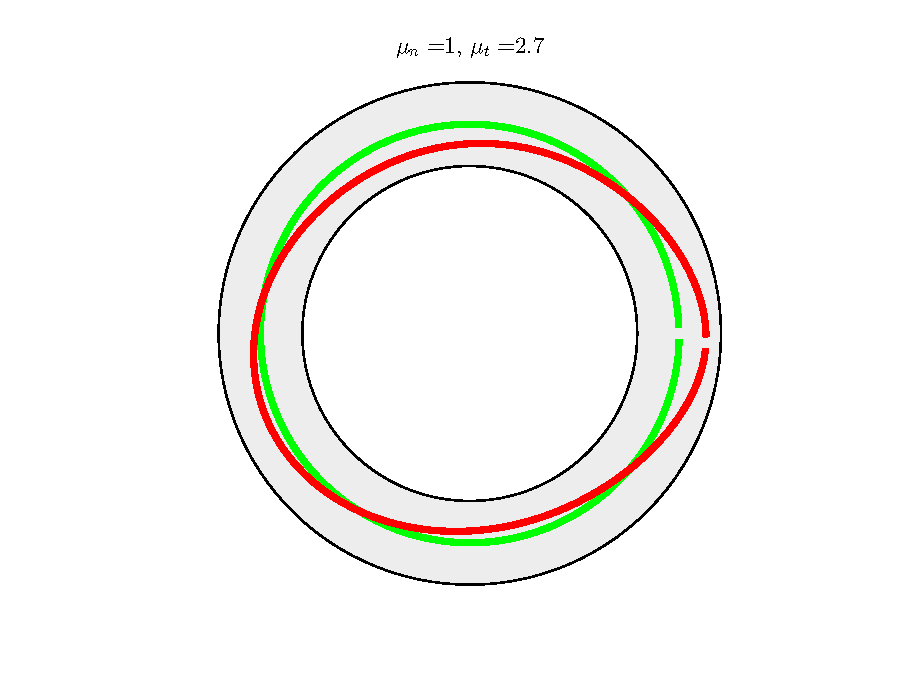
\includegraphics[scale=0.7]{graficos/circular/trayectoria3}
\end{figure}
\end{frame}
\begin{frame}
\begin{figure}[h!]
\begin{tabular}{cc}
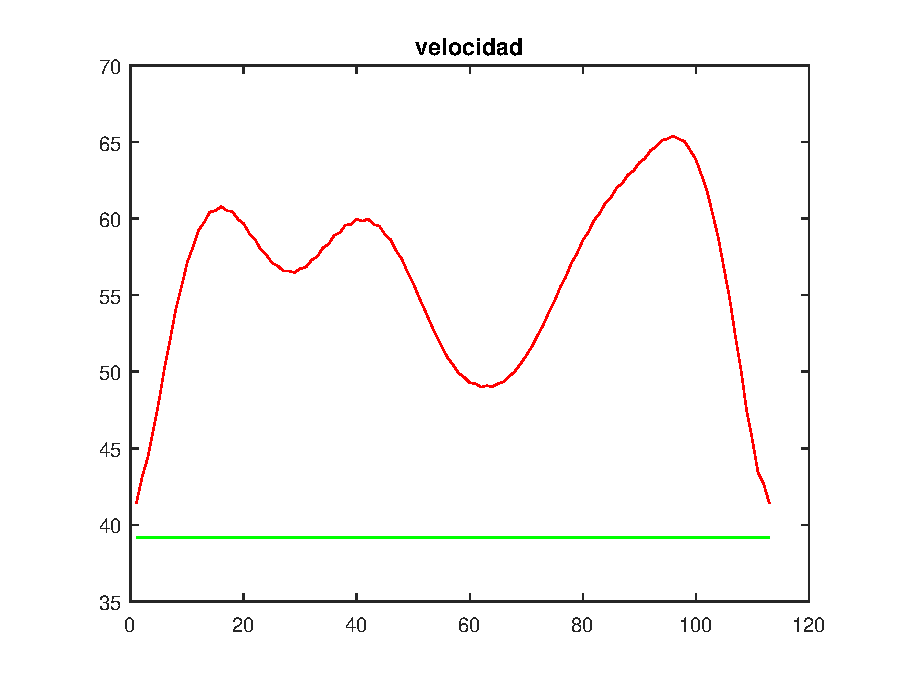
\includegraphics[scale=0.36]{graficos/circular/velocidad3} &
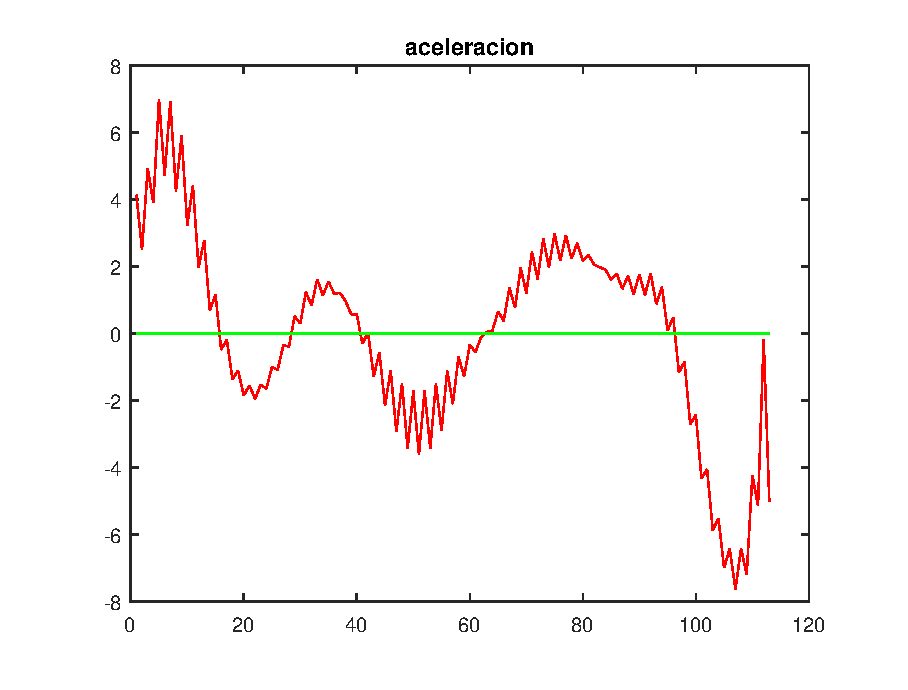
\includegraphics[scale=0.36]{graficos/circular/aceleracion3}
\end{tabular}

\label{circ3}
\end{figure}


\end{frame}

\subsection{Pista cuadrada}
\begin{frame}





\begin{figure}[h!]
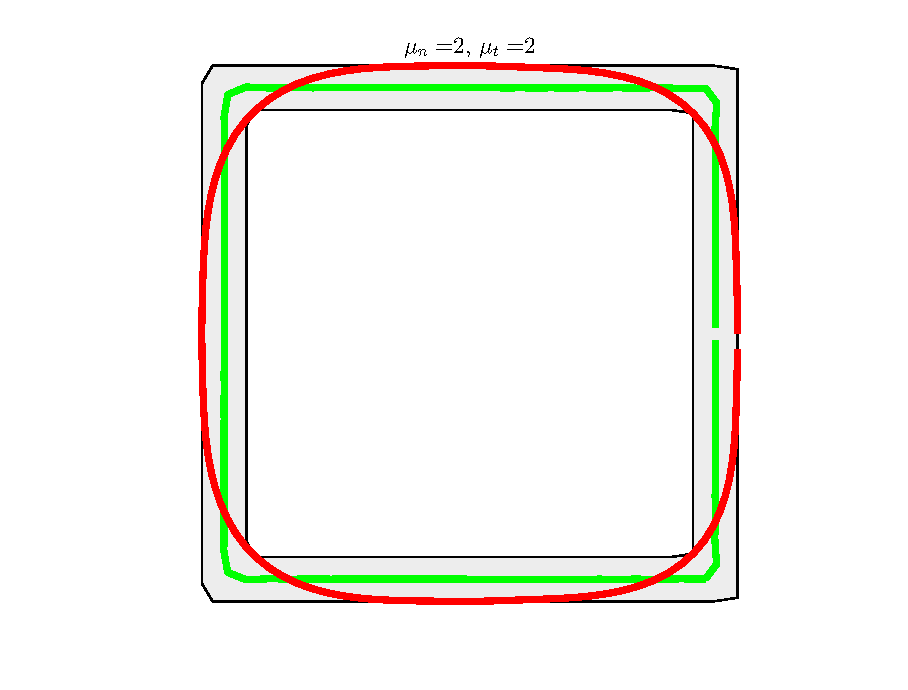
\includegraphics[scale=0.7]{graficos/cuadrada/trayectoria}
\end{figure}
\end{frame}
\begin{frame}
\begin{figure}[h!]
\begin{tabular}{cc}
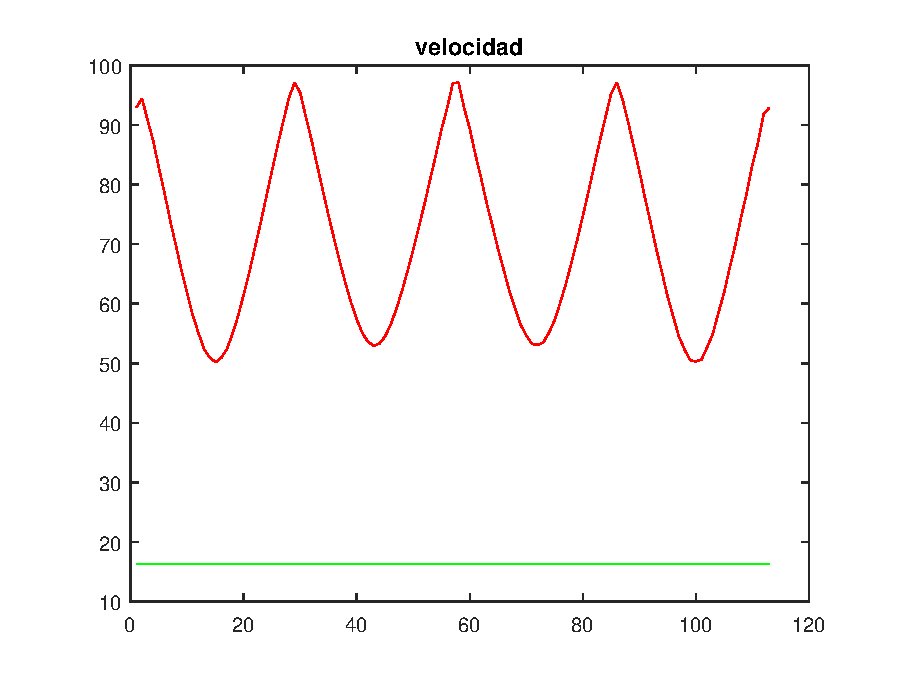
\includegraphics[scale=0.36]{graficos/cuadrada/velocidad.eps} &
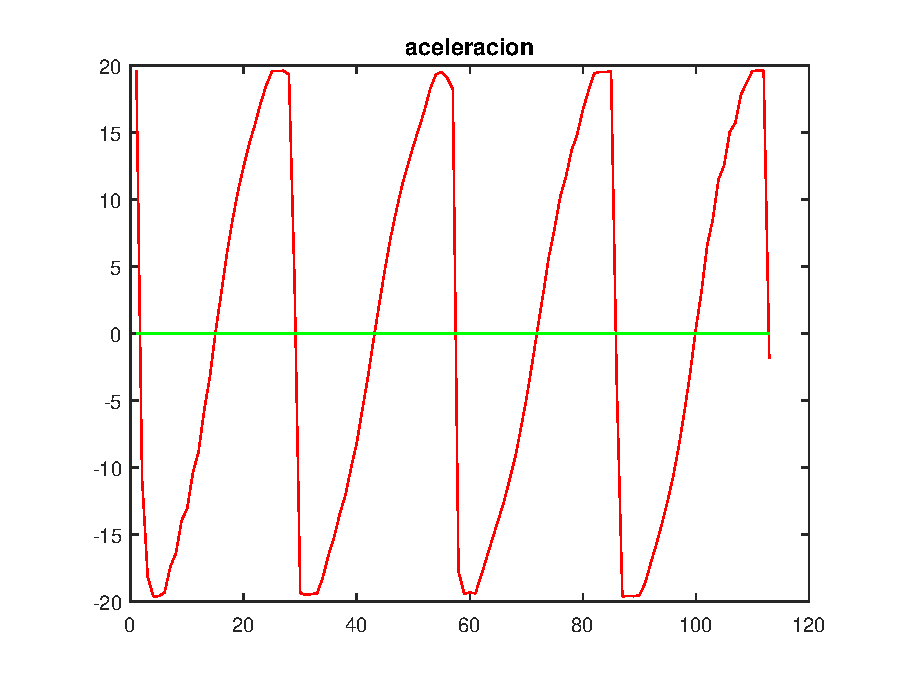
\includegraphics[scale=0.36]{graficos/cuadrada/aceleracion.eps}
\end{tabular}

\label{cuadrada}
\end{figure}


\end{frame}




\subsection{Pista irregular}

\begin{frame}

\begin{figure}[h!]
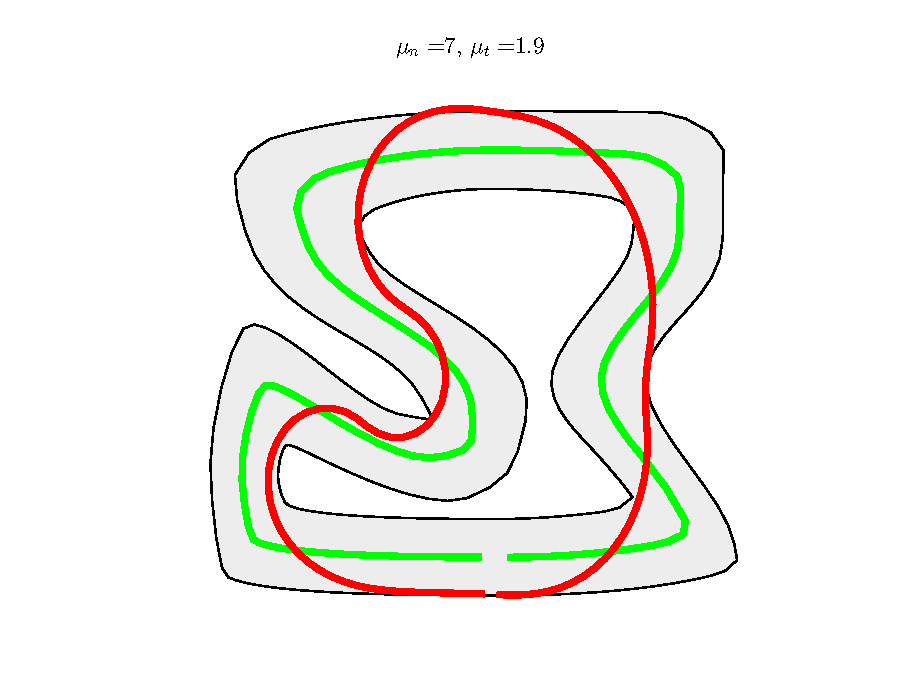
\includegraphics[scale=0.7]{graficos/irregular/trayectoria.eps}
\end{figure}
\end{frame}
\begin{frame}
\begin{figure}[h!]
\begin{tabular}{cc}
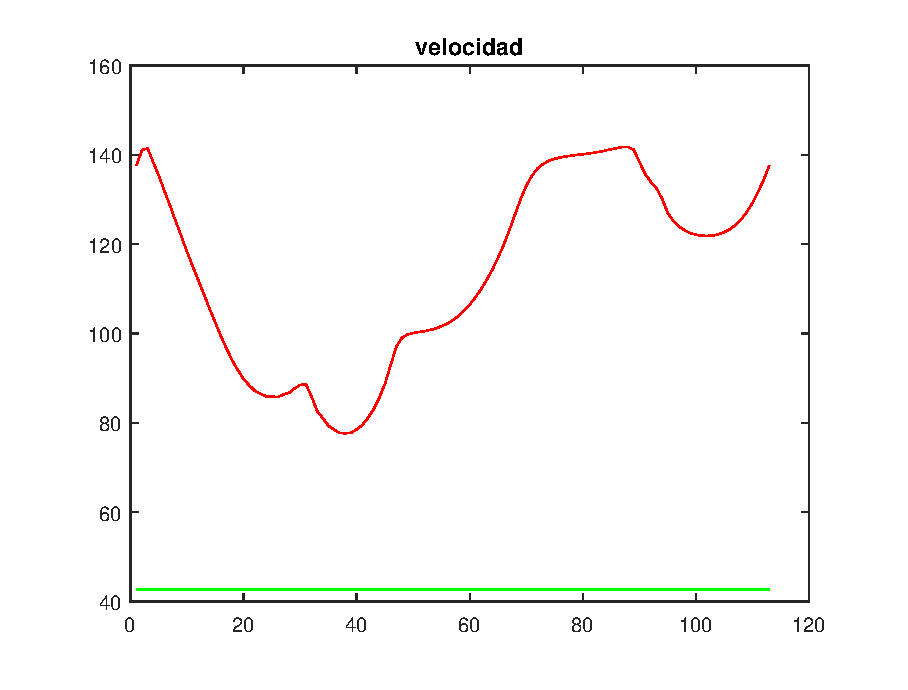
\includegraphics[scale=0.36]{graficos/irregular/velocidad.eps} &
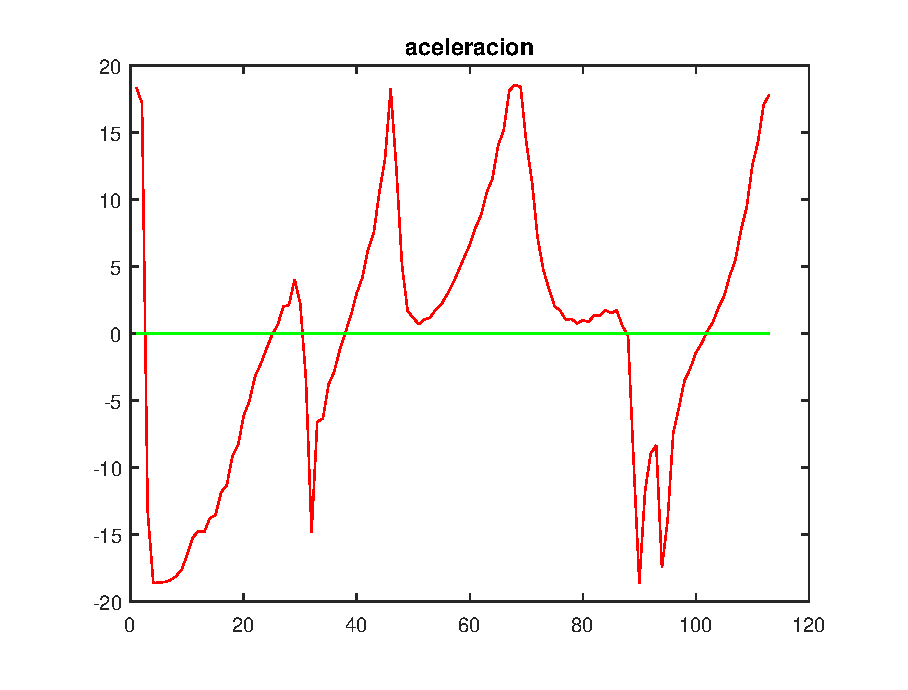
\includegraphics[scale=0.36]{graficos/irregular/aceleracion.eps}
\end{tabular}

\label{cuadrada}
\end{figure}

\end{frame}

\begin{figure}[h!]
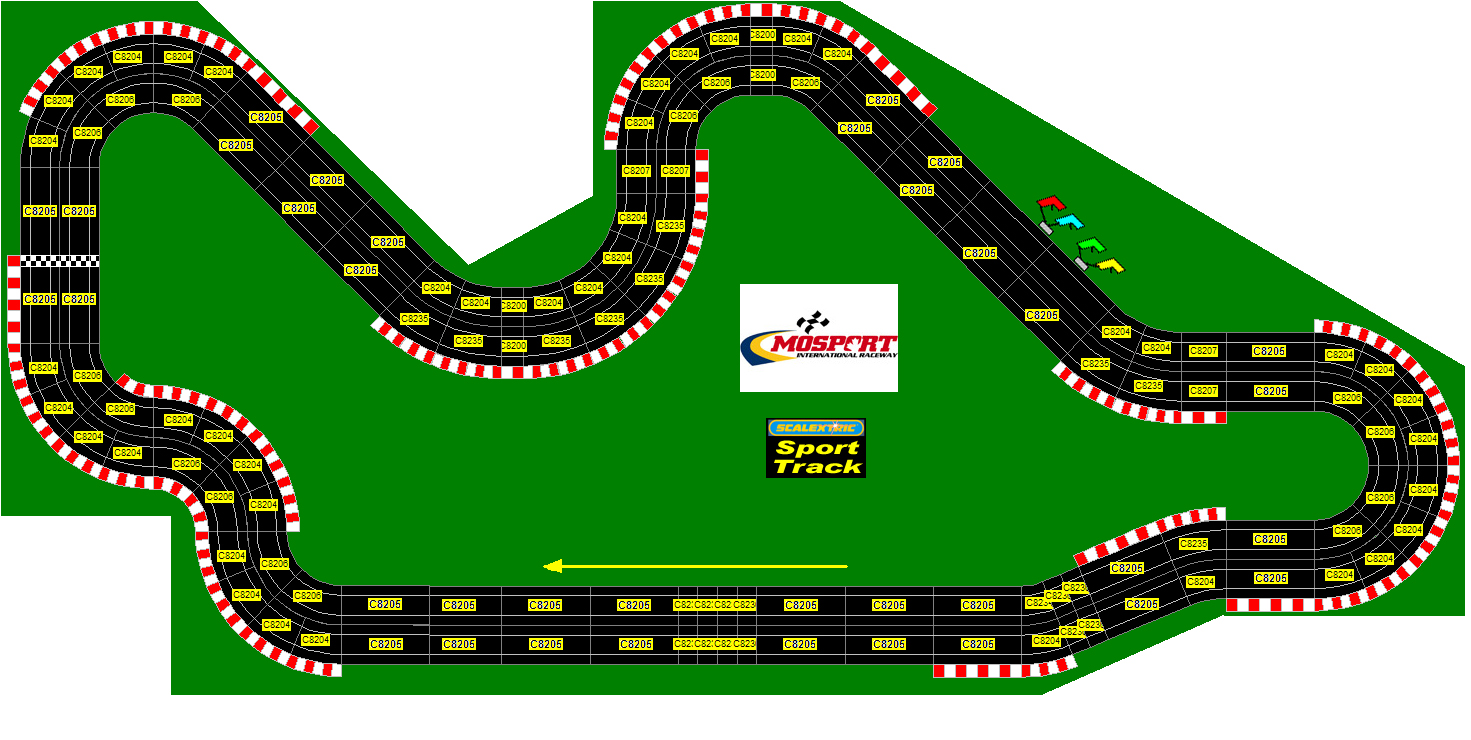
\includegraphics[scale=0.3]{Imagenes/pistacarreragadgadg.jpg}
\caption{Pista en serio.}
\label{pistacarrera}
\end{figure}


\begin{frame}

\begin{figure}[h!]
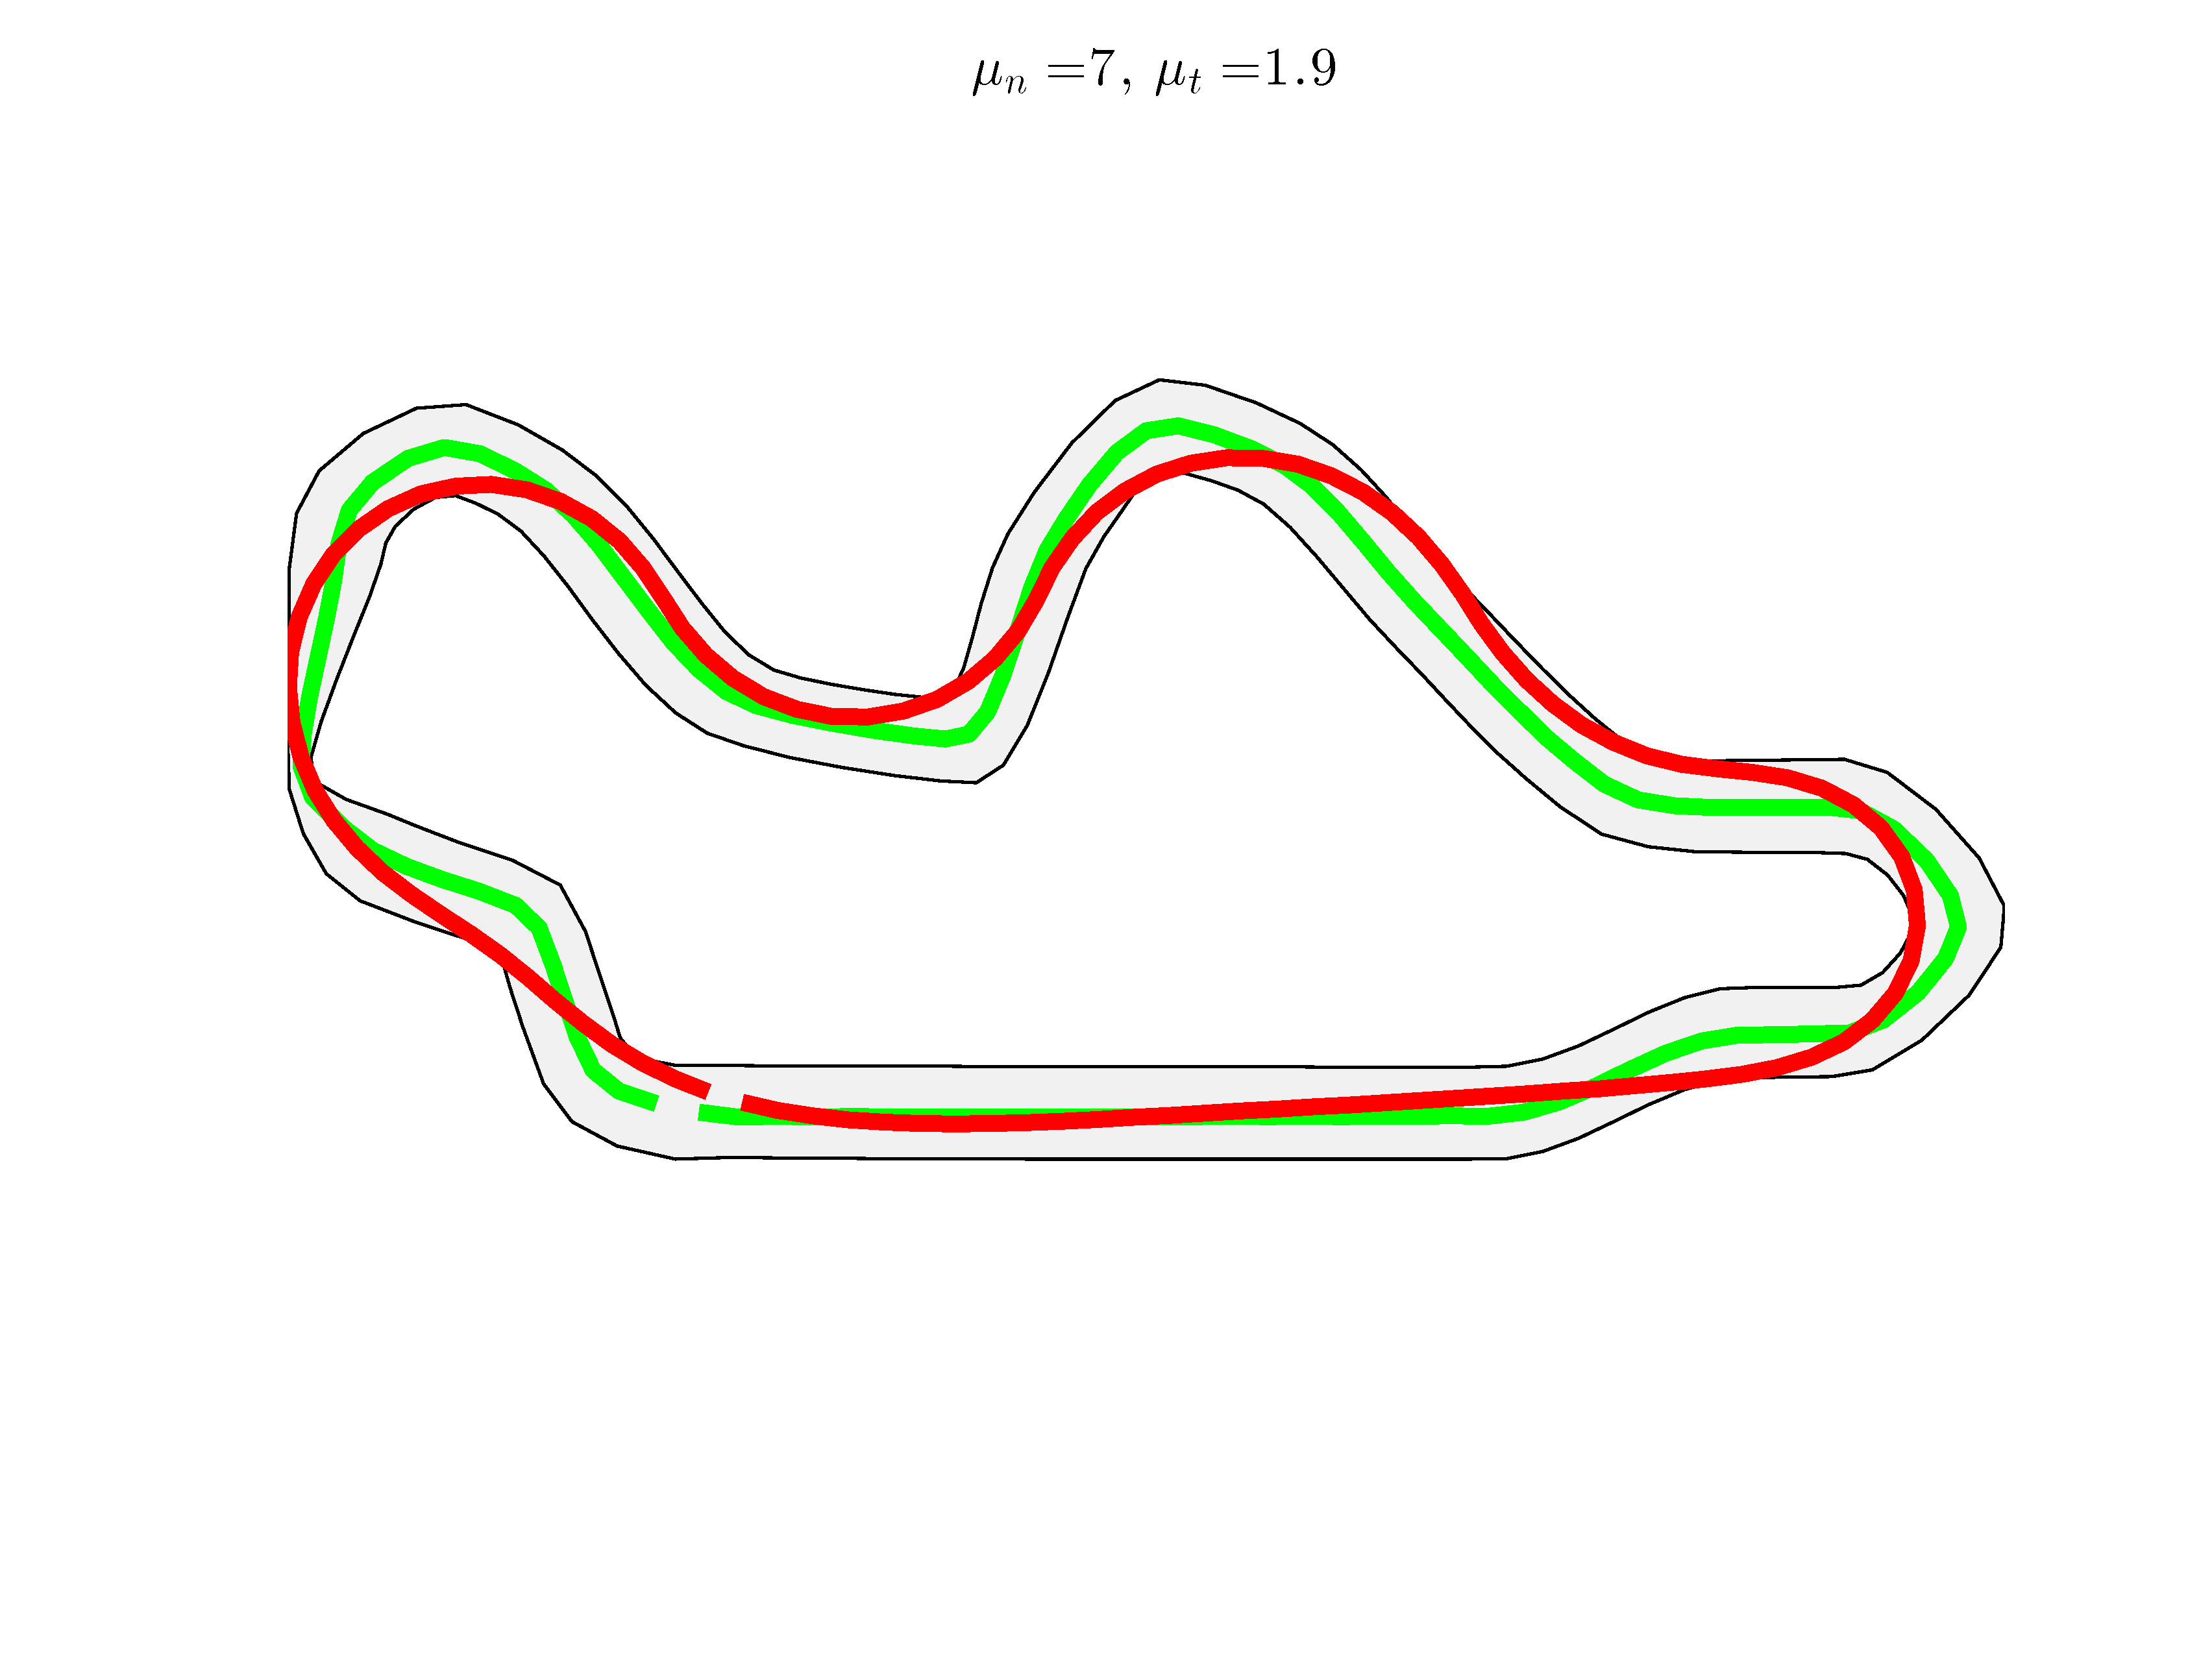
\includegraphics[scale=0.7]{graficos/irregular/trayectoria3}
%\reflectbox{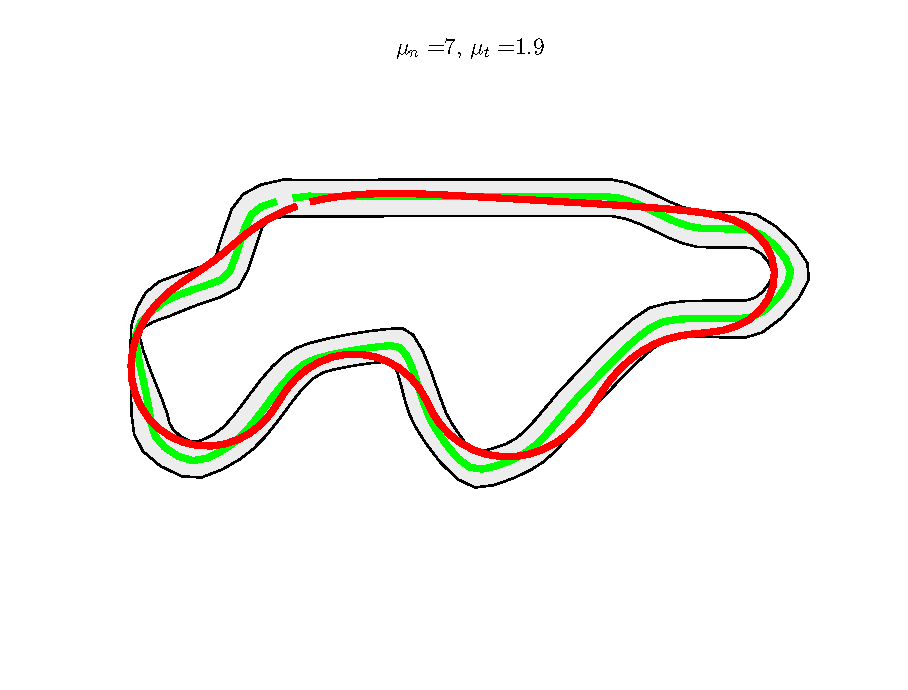
\includegraphics[angle=180,scale=0.7]{graficos/irregular/trayectoria2.eps}}
\end{figure}
\end{frame}
\begin{frame}
\begin{figure}[h!]
\begin{tabular}{cc}
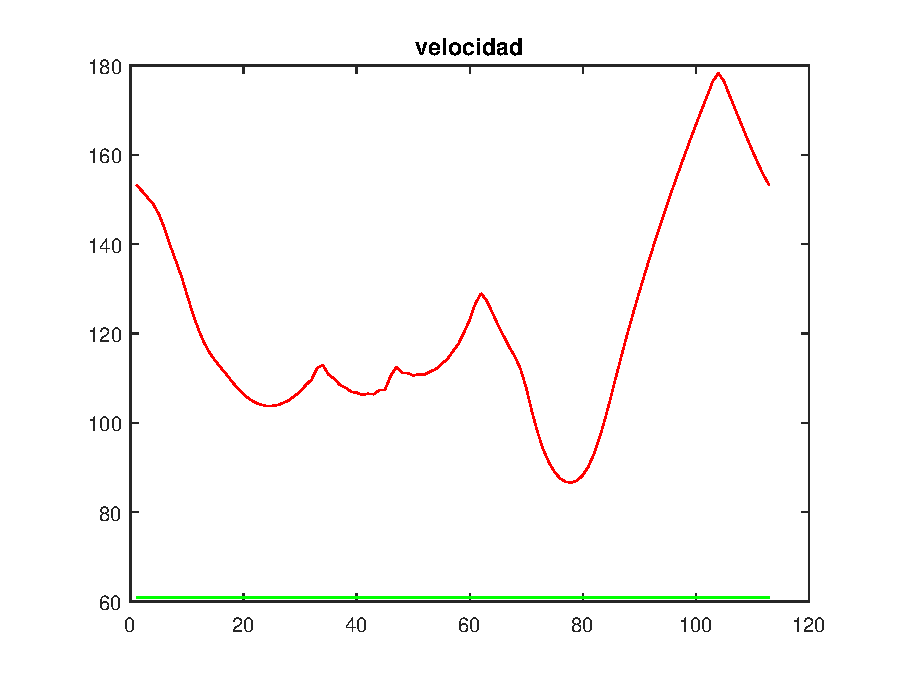
\includegraphics[scale=0.36]{graficos/irregular/velocidad2.eps} &
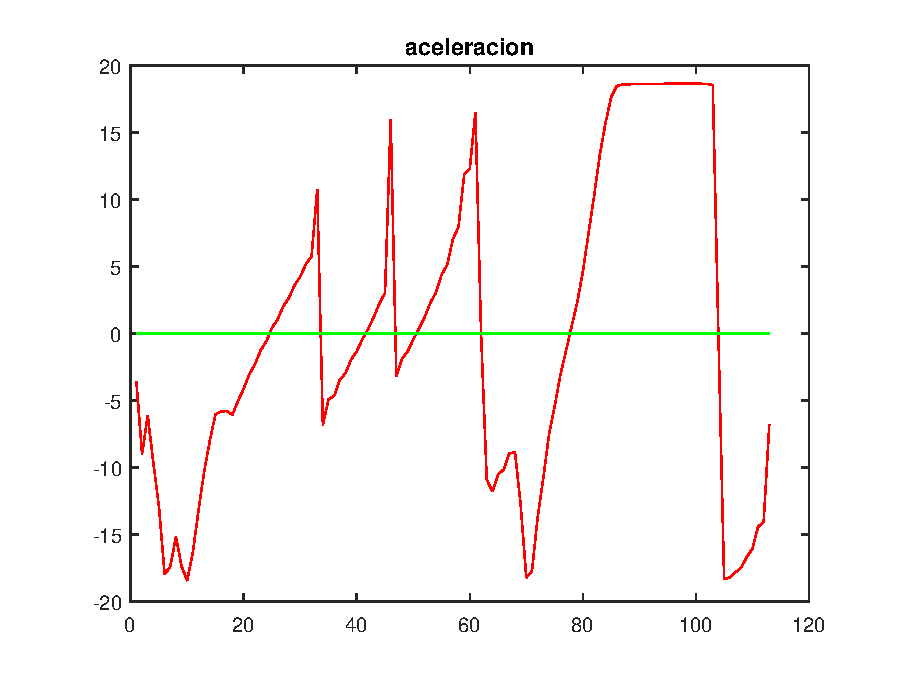
\includegraphics[scale=0.36]{graficos/irregular/aceleracion2.eps}
\end{tabular}

\label{cuadrada}
\end{figure}

\end{frame}
\subsection{Conclusión}
\begin{frame}
\begin{itemize}
\item Se modeló matemáticamente el problema.
\item Se realizó la formulación matemática del mismo.
\item Se programaron los códigos necesarios para el correcto funcionamiento del algoritmo SQP de MATLAB.
\item Se obtuvieron resultados computacionales satisfactorios.
\end{itemize}





% De acuerdo a lo realizado en este trabajo, se puede concluir que se logró el objetivo de plantear y resolver el problema de optimización propuesto, es decir, se encontró una manera de obtener una trayectoria óptima, en un circuito cerrado. Además el código programado también provee la aceleración tangencial y la rapidez.

% El trabajo puede ser utilizado para cualquier circuito de carreras, sólo es necesario dar las coordenadas de las pistas. Sin embargo puede tener diversos usos, como por ejemplo optimizar el recorrido en líneas de producción de fábricas, sólo habría que modificar el problema planteando la correspondiente ecuación de restricción de fricción (ya no necesariamente sería una elipse).
\end{frame}




\begin{frame}

\begin{figure}[h!]
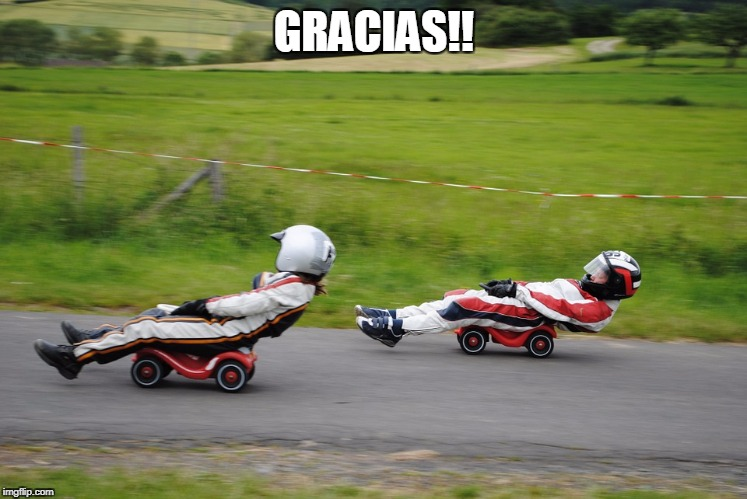
\includegraphics[scale=0.38]{Imagenes/littlecar.jpg}

\end{figure}


\end{frame}

\begin{frame}

\begin{figure}[h!]

\includegraphics[scale=0.57]{Imagenes/homerfinal.jpg}
\end{figure}


\end{frame}








\end{document}








